\documentclass[UTF8]{article}
\usepackage{bm}
\usepackage{amsmath}
\usepackage{cases}
\usepackage{cite}
\usepackage{graphicx}
\usepackage[margin=1in]{geometry}
\geometry{a4paper}
\usepackage{fancyhdr}
\usepackage{array}
\pagestyle{fancy}
\usepackage{wrapfig}
\fancyhf{}
\usepackage{float}  %设置图片浮动位置的宏包
\usepackage{subfigure}
\usepackage{caption}
\usepackage{booktabs}
\usepackage{listings}
\usepackage{xcolor}
\usepackage{multirow}
\lstset{numbers=left, %设置行号位置
	numberstyle=\tiny, %设置行号大小
	keywordstyle=\color{blue}, %设置关键字颜色
	commentstyle=\color[cmyk]{1,0,1,0}, %设置注释颜色
	frame=single, %设置边框格式
	escapeinside=``, %逃逸字符(1左面的键),用于显示中文
	breaklines, %自动折行
	extendedchars=false, %解决代码跨页时,章节标题,页眉等汉字不显示的问题
	xleftmargin=2em,xrightmargin=2em, aboveskip=1em, %设置边距
	tabsize=4, %设置tab空格数
	showspaces=false %不显示空格
}

\title{Curie Point and Hysteresis Line Measurements of Magnetic Materials}
\author{by 22 Artificial Intelligence ChenxuZhang}
\date{2023.11.15}
\pagenumbering{arabic}

\begin{document}
	
	\fancyhead[L]{ChenxuZhang}
	\fancyhead[R]{ID 202264691028}
	\fancyfoot[C]{\thepage}
	
	\maketitle
	\tableofcontents
	\newpage
	
	\section{Abstract}
Magnetic materials play a pivotal role in various scientific and technological applications, the Curie point represents a critical temperature at which magnetic materials undergo a phase transition from ferromagnetic to paramagnetic behavior. Complementing the investigation of the Curie point is the exploration of hysteresis loops, which provide insights into the dynamic response of magnetic materials to varying external magnetic fields. Hysteresis loops illustrate the relationship between magnetization and applied magnetic field during cycles of magnetization and demagnetization. Parameters such as saturation magnetization and coercivity extracted from these loops offer valuable information about a material's magnetic behavior and performance.

 This combined exploration of the Curie point and hysteresis loop serves as a comprehensive study into the magnetic properties of materials, offering a foundation for further research and technological applications. The outcomes of these experiments not only deepen our understanding of magnetic behavior but also contribute to the development of advanced magnetic materials for diverse technological advancements.
 
	
\section{Purpose of the experiment}
   $\bm{A}$.Utilize an oscilloscope to observe the magnetization and demagnetization processes of ferromagnetic materials.\\
   $\bm{B}$.Plot the fundamental magnetization curve of the sample, drawing the B-H curve and the reverse -H curve.\\
   $\bm{C}$.Chart the hysteresis loop of the sample and determine parameters such as $H, B$, and $\Delta B$.\\
   $\bm{D}$.Determine the Curie point temperature of the ferromagnetic material sample.\\
   $\bm{E}$.Based on the hysteresis loop of the sample, estimate its magnetic hysteresis loss.
   
	\section{Experimental apparatus}
    HLD-CZJ-II Magnetic Material Curie Point and Hysteresis Loop Measurement Experimental Apparatus, digital oscilloscope.
    
	\begin{figure}[H]
	    	\centering
	    	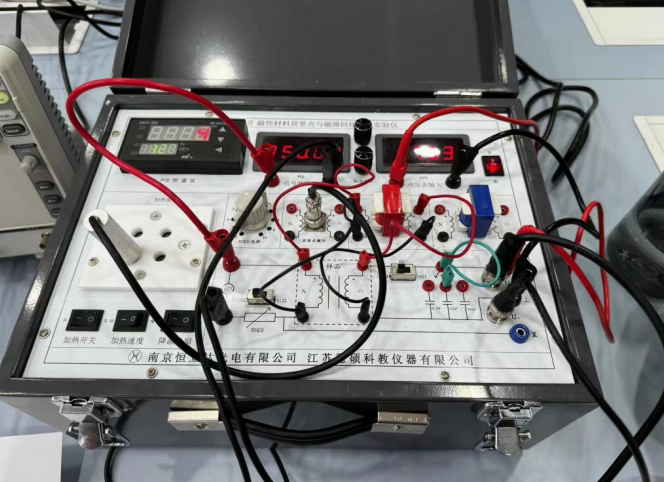
\includegraphics[clip,scale=0.9,trim={0 0 0 0}]{fig/fig1.png}
	        \caption{HLD-CZJ-II Magnetic Material Curie Point and Hysteresis Loop Measurement Experimental Apparatus}
	        \label{figure.1}
    \end{figure}    
    
    \begin{itemize}
        \item \textbf{HLD-CZJ-II Magnetic Material Curie Point and Hysteresis Loop Measurement Experimental Apparatus:}
            \begin{itemize}
                \item Designed for studying magnetic materials, this apparatus enables precise measurements of the Curie Point and Hysteresis Loop.
                \item Equipped with advanced sensors and control mechanisms, allowing accurate data collection and analysis.
                \item Provides a controlled environment for experiments, ensuring reliable and repeatable results.
                \item Features user-friendly interfaces for ease of operation and efficient experimentation.
                \item Ideal for research and educational purposes in the field of magnetic material properties.
            \end{itemize}
            
        \item \textbf{Digital Oscilloscope:}
            \begin{itemize}
                \item A versatile electronic instrument used for visualizing and analyzing varying signal voltages over time.
                \item Employs digital technology for high precision and enhanced functionality.
                \item Offers multiple channels for simultaneous signal monitoring.
                \item Equipped with a user-friendly interface and controls for easy operation and data interpretation.
                \item Widely utilized in electronics, physics, and engineering applications for waveform analysis.
            \end{itemize}
    \end{itemize}
    
	\begin{figure}[H]
	    	\centering
	    	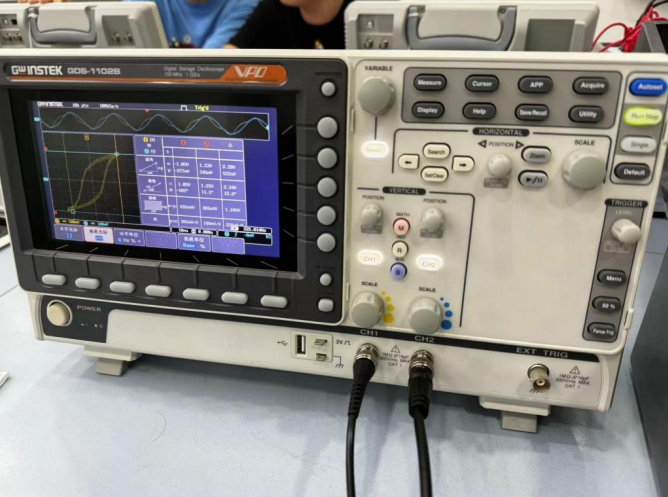
\includegraphics[clip,scale=0.9,trim={0 0 0 0}]{fig/fig2.png}
	        \caption{digital oscillosope}
	        \label{figure.1}
    \end{figure}        
    
        
	\section{Experimental principles}   
    \subsection{Magnetization of ferromagnetic material}
    Ferromagnetic materials are a class of materials characterized by distinct properties and versatile applications. Iron, cobalt, nickel, and numerous alloys, as well as iron-containing oxides, all fall under the category of ferromagnetic materials. One defining characteristic is their ability to be strongly magnetized under the influence of an external magnetic field, resulting in a high magnetic permeability. Another notable feature is their hysteresis behavior, wherein the material retains a certain magnetization state even after the magnetic field ceases.
   
   When ferromagnetic materials are placed within a magnetic field generated by an electric current, the magnetic field becomes significantly enhanced. In this scenario, the magnetic induction strength within the ferromagnetic material is much greater than the induction strength generated solely by the electric current, often increasing by factors of hundreds or even thousands. The relationship between the internal magnetic field strength $(H)$ and magnetic induction strength $(B)$ within ferromagnetic materials is described by the following relationship:
   \begin{eqnarray}
   B = \mu H
   \end{eqnarray}
   \begin{figure}[H]
   	    	\centering
   	    	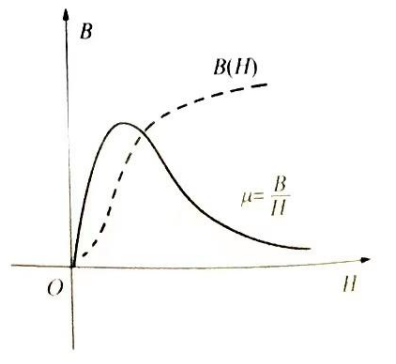
\includegraphics[clip,scale=0.9,trim={0 0 0 0}]{fig/fig3.png}
   	        \caption{B-H curve and u-H curve}
   	        \label{figure.1}
       \end{figure}  
   
   For ferromagnetic materials, the magnetic permeability $(μ)$ is not a constant but a physical quantity that changes with variations in the magnetic field strength $(H)$; that is, $\mu = f(H)$ represents a nonlinear function. As illustrated in Figure, both the relationships between $H$ and $B$, and $H$ and $\mu$ exhibit nonlinearity for ferromagnetic materials. 
   
   The magnetization process for ferromagnetic materials can be described as follows: the state before magnetization is termed the demagnetized state. In this state, if a magnetizing field, gradually increasing in magnitude, is applied to the ferromagnetic material, the internal magnetic field strength $(H)$ and magnetic induction strength $(B)$ within the material also increase accordingly. The $B-H$ variation curve is depicted in Figure. However, when $H$ increases to a certain value $(H_s)$, $B$ almost ceases to increase with further increments in $H$, indicating saturation of magnetization. The magnetization curve from demagnetization to saturation magnetization is referred to as the material's initial magnetization curve, as illustrated by the OS curve in Figure.
   
   \subsection{Hysteresis loop}
   After the magnetization of ferromagnetic materials reaches saturation, if the magnetizing field is reduced, the internal values of $B$ and $H$ within the ferromagnetic material decrease. However, the process of reduction does not follow the OS segment of the magnetization curve. As depicted in Figure, when the magnetizing field is eliminated and $H$ returns to zero (point h in the figure), the magnetic induction strength maintains a certain value, denoted as $B = B_r$ , referred to as residual magnetization (or remanent magnetic induction strength).
   
   \begin{figure}[H]
   	    	\centering
   	    	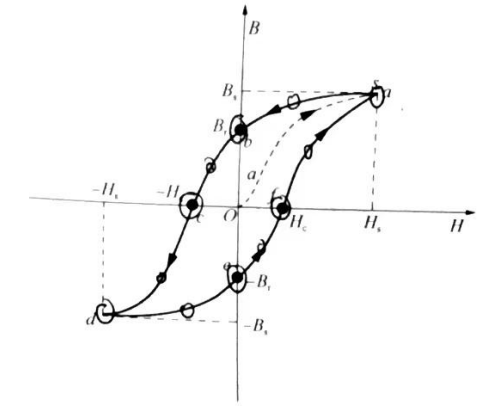
\includegraphics[clip,scale=0.9,trim={0 0 0 0}]{fig/fig4.png}
   	        \caption{Initial magnetization curve and hysteresis loop}
   	        \label{figure.1}
       \end{figure}  
   
   To reduce the magnetic induction strength B of magnetized ferromagnetic material to zero, it is necessary to apply a reverse magnetic field and gradually increase it. When the internal reverse magnetic field strength within the ferromagnetic material reaches $H = -H_c$ (as indicated in point $d$ in Figure), the magnetic induction strength $B$ becomes zero, achieving demagnetization. The curve segment be in Figure is referred to as the demagnetization curve, and $H$ is termed coercivity.
   
   As shown in Figure, when $H$ changes sequentially in the order of $O->H_s->O->-H_c- >-H_s->O->H_c->H_s$, $B$ correspondingly changes in the order of $O->B_s->B_r->O->-B_s->-B_r->O- >B_s$. The curve segment $Oa$ in the figure is known as the initial magnetization curve, and the closed loop formed by the aforementioned variation process is called the hysteresis loop (abedefa). 
   
   From the above, the following conclusions can be drawn:
   
   \begin{itemize}
       \item When \(H = 0\), \(B\) is not zero, indicating the presence of a residual magnetic induction strength \(B_r\), commonly referred to as remanence.
       \item To completely demagnetize ferromagnetic material, i.e., \(B = 0\), a reverse magnetic field \(-H\) must be applied. The strength of this magnetic field, \(H_c\), is termed the coercive force of the ferromagnetic material.
       \item The change in \(B\) always lags behind the change in \(H\); that is, when \(H\) decreases to 0, \(B\) is not zero, and \(B\) becomes zero only when \(H\) reverses to a certain value. This phenomenon is known as magnetic hysteresis.
       \item From the image of the hysteresis loop, it is evident that for a specific value of \(H\), the \(B\) value within the ferromagnetic material may vary, and the \(B\) value is related to the magnetic history of the material.
       \item When the initial state is \(H = 0\), \(B = 0\), and the strength of the field is periodically changed, a family of hysteresis loops with increasing areas can be obtained during the monotonic increase of the field. The hysteresis loop with the maximum area is referred to as the saturation hysteresis loop, as shown in Figure.
       \item Due to the irreversibility of the magnetization process in ferromagnetic materials and their characteristic of residual magnetization, it is imperative to demagnetize the ferromagnetic material before determining magnetization curves and hysteresis loops. This ensures that when the external magnetic field $H = 0$, the magnetic induction strength $B$ is also $0$. Furthermore, the magnetizing current during the experimental process should only increase monotonically (up to bidirectional saturation) or decrease, it should not alternate between increase and decrease.
   \end{itemize}
   
      \begin{figure}[H]
             \begin{minipage}[t]{0.5\linewidth}
                \centering
                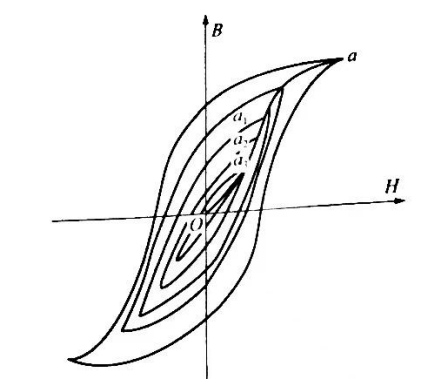
\includegraphics[clip,scale=0.9,trim={0 0 0 0}]{fig/fig5.png}
                \label{figure.11}
                \caption{Hysteresis loop}
             \end{minipage}
             \begin{minipage}[t]{0.5\linewidth}
                \centering
                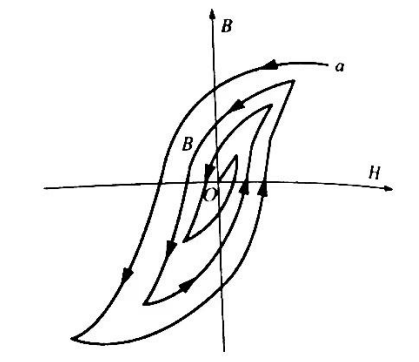
\includegraphics[clip,scale=0.9,trim={0 0 0 0}]{fig/fig6.png}
                \label{figure.12}
                \caption{Demagnetization curve}
             \end{minipage}   	  
          \end{figure}  
          
    In theory, to eliminate residual magnetization $B$, it is sufficient to pass a reverse magnetizing current to make the applied magnetic field exactly equal to the coercive force of the ferromagnetic material. However, in practice, the magnitude of the coercive force is often unknown, making it challenging to determine the size of the demagnetizing current. Insights can be derived from the hysteresis loop: if the ferromagnetic material is first magnetized to magnetic saturation and then the direction of the magnetizing current is continuously changed while gradually reducing the amplitude of the magnetizing current until it reaches $0$ (i.e., the magnetizing current becomes a decreasing AC current), the magnetization process of the material forms a series of gradually shrinking circular curves ultimately converging to the origin, as shown in Figure. When H decreases to $0, B$ simultaneously drops to $0$, achieving complete demagnetization. 
    
    Experimental results indicate that after multiple cycles of repeated magnetization, the quantity relationship between B and H forms a stable closed "hysteresis loop." This loop is commonly used to represent the magnetic properties of the material. The process of repeated magnetization is referred to as "magnetic annealing." In this experiment, using alternating current ensures sufficient "magnetic annealing" for each state, allowing the hysteresis loop to be obtained at any time. 
    
    The line connecting the origin $0$ and the vertices a, $a, ..., a$ of each hysteresis loop in Figure is referred to as the basic magnetization curve of the ferromagnetic material. Different ferromagnetic materials have different basic magnetization curves. To ensure the repeatability of the magnetic characteristics of the sample, meaning that the measured basic magnetization curves all start from the original state $(H = 0, B = 0)$, demagnetization must be performed before measurement to eliminate residual magnetism in the sample. 
    
    During the measurement of the basic magnetization curve, each magnetization state must undergo sufficient "magnetic annealing"; otherwise, the obtained B-H curve will be the initial magnetization curve, and the two should not be confused.     
   
    \subsection{The principle of oscilloscope displaying B-H curve}
    The experimental circuit is depicted in Figure. The ferromagnetic material under investigation (the test sample) is an EI-type silicon steel sheet. $N$ represents the primary excitation winding, and $n$ is the secondary measurement winding established for measuring the magnetic induction strength $B. R$ is the sampling resistor for the excitation current, converting the current into voltage. Let the alternating excitation current passing through N berepresented by $I$. According to Ampere's circuital law, the magnetizing field strength of the sample is determined by the equation:
       \begin{figure}[H]
       	    	\centering
       	    	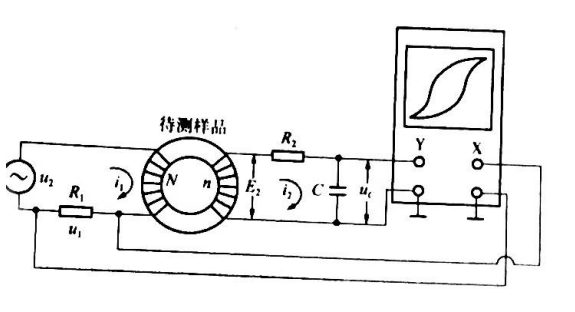
\includegraphics[clip,scale=0.9,trim={0 0 0 0}]{fig/fig7.png}
       	        \caption{Experimental circuit}
       	        \label{figure.1}
           \end{figure}  
    
    \begin{eqnarray}
    H = \frac{Ni_1}{L}
    \end{eqnarray}
    
    In the formula, L is the average sipping length of the sample. Because of $i_1 = \frac{u_1}{R_1}$,so:
    \begin{eqnarray}
    H = \frac{Ni_1}{L} = \frac{N}{LR_1}u_1
    \end{eqnarray}
    $N$, $L$, and $R_1$ are known constants, so H can be determined from the given $u$.
    
    Under alternating magnetic fields, the instantaneous value of the magnetic induction strength $B$ of the sample is determined by the secondary measurement winding n and the known constants $R_2$ and $C_2$ in the circuit. According to Faraday's law of electromagnetic induction, the magnitude of the induced electromotive force generated in the measurement coil, due to the variation of magnetic flux in the sample, is given by:
    
    \begin{eqnarray}
    \varepsilon_{2}=\mathrm{n} \frac{\mathrm{d} \varphi}{\mathrm{dt}}
    \end{eqnarray}
    \begin{eqnarray}
    \varphi=\frac{1}{\mathrm{n}} \int \varepsilon_{2} \mathrm{dt}
    \end{eqnarray}
    \begin{eqnarray}
    \mathrm{B}=\frac{\varphi}{\mathrm{S}}=\frac{1}{\mathrm{nS}} \int \varepsilon_{2} \mathrm{dt} 
    \end{eqnarray}
    
    S represents the cross-sectional area of the sample.
    If we neglect self-induced electromotive force and circuit losses, the circuit equation is given by:
    \begin{eqnarray}
    \varepsilon_{2}=\mathrm{i}_{2} \mathrm{R}_{2}+\mathrm{u}_{\mathrm{c}} 
    \end{eqnarray}
    
    In the equation, $i_2$ represents the induced current, and $u_c$ represents the voltage across the integrating capacitor $C$. Assuming that within a time period $\Delta t$, the charge accumulated due to the charging current $i_2$ into the capacitor $C$ is denoted as $Q$,then:
    \begin{eqnarray}
    \mathrm{u}_{\mathrm{c}}=\frac{\mathrm{Q}}{\mathrm{C}}
    \end{eqnarray}
    
    Therefore:
    \begin{eqnarray}
    \varepsilon_{2}=\mathrm{i}_{2} \mathrm{R}_{2}+\frac{\mathrm{Q}}{\mathrm{C}} 
    \end{eqnarray}
    
    If sufficiently large values are chosen for R2 and C such that $i_2R_2 >> \frac{Q}{C}$,then:
    \begin{eqnarray}
    \varepsilon_{2} = i_2 R_2
    \end{eqnarray}
    
    Because:
    \begin{eqnarray}
    \mathrm{i}_{2}=\frac{\mathrm{dQ}}{\mathrm{dt}}=\mathrm{C} \frac{\mathrm{du}_{\mathrm{c}}}{\mathrm{dt}}
    \end{eqnarray}
    
    So:
    \begin{eqnarray}
    \varepsilon_{2}=\mathrm{CR}_{2} \frac{\mathrm{du}_{\mathrm{c}}}{\mathrm{dt}}
    \end{eqnarray}
    
    Then, we can obtain:
    \begin{eqnarray}
    \mathrm{B}=\frac{\mathrm{CR}_{2}}{\mathrm{nS}} \mathrm{u}_{\mathrm{c}}
    \end{eqnarray}
    
    In the above equation, $C, R_2, n$ and $S$ are both known constants, so $B$ can be determined by $u_c$.
    
     In summary, by connecting $u1 (uH)$ and $uC (uB)$ to the "$X$ input" and "$Y$ input" of an oscilloscope, respectively, one can observe the dynamic hysteresis loop of the sample.Connecting to a digital voltmeter allows for the direct measurement of $u1(uH)$ and $uC(uB)$, facilitating the plotting of the $B-H$ curve. Through calculations, parameters such as the saturation magnetic induction strength $R_s$, residual magnetization $R_r$, coercive force $H_c$, hysteresis loss BH, and magnetic permeability μ of the sample can be determined.
     
     Under the mentioned conditions, the amplitude of $u_C$ is very small, and it cannot directly generate a hysteresis loop of suitable size for observation. Therefore, it is necessary to amplify $u_C$ through the Y-axis amplifier of the oscilloscope before sending it to the Y-axis deflection plate. This requires that, within the frequency range of the experimental magnetic field, the amplification factor of the amplifier must be stable and not introduce significant phase distortion. In reality, it is challenging for the oscilloscope to fully meet this requirement, and distortions like the one shown in Figure often occur during the experiment.
     
     To mitigate such distortions during observation, the X-axis input should be set to "AC" mode, the Y-axis input should be set to "DC" mode, and appropriate values for $R_1$ and the resistor $R_2$ in the circuit, as well as the amplitude of the signal source, should be selected. This can help avoid distortions and achieve the optimal hysteresis loop shape.
    
        \begin{figure}[H]
           	    	\centering
           	    	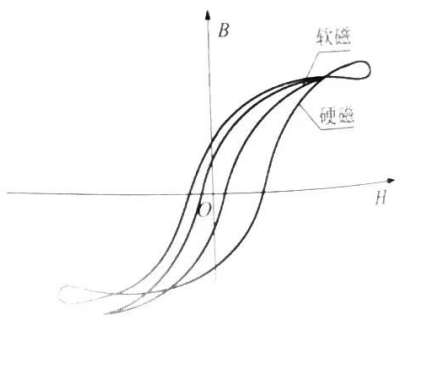
\includegraphics[clip,scale=0.9,trim={0 0 0 0}]{fig/fig8.png}
           	        \caption{Graphic distortion caused by circuit}
           	        \label{figure.1}
               \end{figure}  
               
     In this manner, over one cycle of the magnetizing current variation, a complete hysteresis loop will be traced on the oscilloscope screen. By appropriately adjusting the $X$ and $Y$ axis gains on the oscilloscope and gradually increasing the output voltage of the signal generator, you can observe an expanding hysteresis loop on the screen. Record the coordinates of its positive vertices step by step, and connect them into a smooth curve on graph paper. This process yields the basic magnetization curve of the sample.          
               
     \subsection{Curie point and its measurement}          
      Ferromagnetic materials exhibit microscopic mechanisms related primarily to two factors. Firstly, the magnetism of ferromagnetic materials originates mainly from the electron spin magnetic moments. Secondly, in ferromagnetic materials at room temperature, there are numerous spontaneously magnetized microscopic regions known as magnetic domains. So, how are these magnetic domains formed? And how are they affected by an external magnetic field?
      
      Modern physics theories suggest that there exists a very strong exchange coupling interaction between adjacent electrons. This interaction causes the spin magnetic moments of electrons to align parallel to each other, forming tiny regions of spontaneous magnetization that reach a saturated state. The volume of these regions is approximately $10^{-12}$ to $10^{-8} m^3$, and they are referred to as magnetic domains. 
      
      When the external magnetic field is zero $(H=0)$ and the material is demagnetized (in a demagnetized state), the orientations of different magnetic domains are random, and the probabilities in all directions are equal. Therefore, the average magnetic moment within any macroscopic region of the ferromagnetic material is zero, and the material does not exhibit magnetism $(B=0)$. When an external magnetic field is applied, the orientations of different magnetic domains tend to align with the direction of the external magnetic field. The average magnetic moment within any macroscopic region is no longer zero $(B\ne 0)$, and it increases with the magnitude of the external magnetic field (the ferromagnetic material is magnetized). When the external magnetic field increases to a certain value, all the magnetic domains align along the direction of the external magnetic field, and the average magnetic moment within any macroscopic region reaches its maximum value, indicating saturation magnetization. 
      
      From the above process, it can be observed that the magnetization of ferromagnetic materials is the result of the summation of all the electron spin magnetic moments. This characteristic imparts strong magnetism to ferromagnetic materials, and the magnetic permeability $(u)$ of ferromagnetic materials is much greater than that of paramagnetic materials. During the process of diminishing or disappearing external magnetic fields, the effects of thermal motion cause the orientations of magnetic domains to become disorderly again. This leads to a reduction or disappearance of the material's magnetization (demagnetization). However, due to factors such as impurities and internal stresses within the material, the orientations of magnetic domains do not fully recover, resulting in the residual magnetism and hysteresis characteristics of ferromagnetic materials.
      
      Ferromagnetic materials exhibit strong magnetism when magnetized, but this magnetism is temperature-dependent. As the temperature of ferromagnetic substances increases, the intensified thermal motion of metal lattice points affects the arrangement of magnetic domain magnetic moments. At this point, the material still possesses magnetism, but the average magnetic moment decreases with the rise in temperature. However, when the thermal motion, proportional to $kT$, becomes significant enough to disrupt the structure of magnetic domains, the domains disintegrate, and the material's ferromagnetism disappears, transforming into paramagnetic behavior. A series of related ferromagnetic properties, such as high magnetic permeability, hysteresis loop, magnetostriction, etc., all vanish. The corresponding magnetic permeability transforms into the paramagnetic magnetic permeability, changing from significantly greater than 1 to approximately equal to 1. The temperature corresponding to the disappearance of ferromagnetism is called the Curie temperature, abbreviated as the Curie point, denoted by the symbol $T_c$. 
      
      There are generally two methods for measuring the Curie point of ferromagnetic materials. The first method involves observing the changes in the hysteresis loop as the temperature increases. When approaching the Curie point, the hysteresis loop area decreases, and the curve becomes more linear. The temperature corresponding to the point where the loop just disappears is the Curie point. The second method involves plotting the curve of magnetic permeability versus temperature and identifying the Curie point from the curve. Since measuring magnetic permeability directly can be challenging, the Curie point can be determined by plotting the curve of induced electromotive force against temperature. The specific method and analysis are as follows: 
      
      Wind coils $N$ and $n$ on the magnetic ring respectively, and apply excitation current on the $N$ coil, then the effective value of induced electric heat on the $n$ line is:         
      \begin{eqnarray}
      \varepsilon_{eff} = 4.44 fn\Phi_m
      \end{eqnarray}         
      
      In the formula, $f$ is the frequency; $n$ is the number of coil turns; $4.44$ is the instrument constant;$\Phi_m$ is the maximum magnetic flux.   
      \begin{eqnarray}
      \Phi_m = B_m S
      \end{eqnarray}      
      
      $S$ is the cross-sectional area of the magnetic ring; $B_m$ is the maximum magnetic induction intensity, which is the amplitude of the sinusoidal change in magnetic induction intensity.
      
      In addition:
      \begin{eqnarray}
      H = \frac{B}{\mu}
      \end{eqnarray}
      
      $\mu$ is the magnetic permeability, measured in $H/m$ in the SI system. Substitute equations for equations, and obtain:
      \begin{eqnarray}
      \varepsilon_{eff} = 4.44 fn S\mu H_m
      \end{eqnarray}
       
      $H_m$ is the amplitude of the magnetic field intensity, and when the excitation current stabilizes into a sinusoidal variation, $H_m$ is constant. Immediate acquisition:
      \begin{eqnarray}
      \varepsilon_{eff} \propto \mu
      \end{eqnarray}
       
       The temperature of ferromagnetic materials usually reaches the order of $10^3$, while the temperature of paramagnetic materials increases to the Curie point $TC$. When nearby, the induced electromotive force will sharply decrease.
       
       Clearly, we can use the plotted curve of $\varepsilon_{eff}-T$ to determine the temperature TC. Specifically, at the point where the slope of the $\varepsilon_{eff}−T$ curve is maximum, draw a tangent line. The intersection of this tangent line with the x-axis gives the temperature $T_C$, as shown in This is because at the Curie point, there is a sudden change in the magnetic properties of the ferromagnetic material, necessitating the drawing of a tangent at the point of maximum slope. Furthermore, since the ferromagnetic nature has essentially transformed into paramagnetism close to the Curie point, the $\varepsilon_{eff}−T$ curve cannot intersect the x-axis.
       
       \begin{figure}[H]
           	    	\centering
           	    	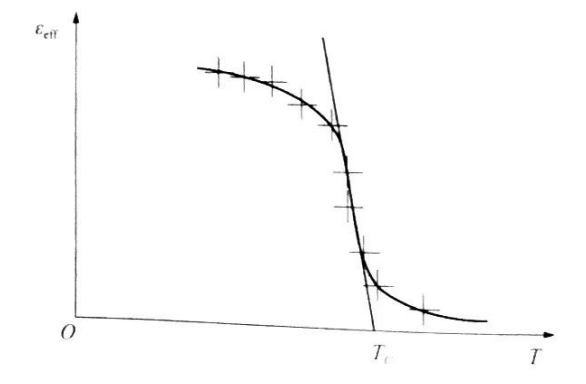
\includegraphics[clip,scale=0.9,trim={0 0 0 0}]{fig/fig9.png}
           	        \caption{Determining the Curie Point by Measuring the Curve of Induced Electromotive Force Changing with Temperature}
           	        \label{figure.1}
               \end{figure}    
               
    \subsection{Hysteresis loss and its measurement}
      During the repeated magnetization process (magnetization - demagnetization - reverse magnetization - demagnetization - remagnetization) of ferromagnetic materials, the variation of B-H forms a hysteresis loop. Microscopic physical movements occur within the magnetic domains of the material, which can be understood as rigid molecular rotations. The continuous cyclic movement manifests externally in the following ways:
      
      \begin{itemize}
          \item Changes in the magnetization direction lead to variations in the material's lattice spacing, causing dimensional changes in the material. This is known as the magnetostriction effect, and the typical length change induced by magnetostriction is on the order of \(10^{-5}\).
          \item In the process of repeated magnetization, the excitation power supply needs to continuously perform work, and the energy transferred is ultimately dissipated in the form of heat. The energy dissipated due to the hysteresis characteristics is referred to as hysteresis loss.
      \end{itemize}
      
      Within one complete magnetization cycle, the hysteresis loss per unit volume of magnetic core is equal to the area enclosed by the hysteresis loop. Soft magnetic materials have narrow hysteresis loops with small values of $B$ and $H$, resulting in relatively low hysteresis loss. These materials are suitable for use as core materials in motors, transformers, and inductors. Hard magnetic materials, on the other hand, have large values of $B$ and $H$, making them suitable for producing permanent magnets. However, their hysteresis loops are broad, and the hysteresis loss is relatively high, making them unsuitable for use in AC circuits.
      
      In summary, at higher frequencies and higher magnetic flux densities, the area enclosed by the hysteresis loop increases, leading to greater hysteresis loss. Theoretically, the hysteresis loss W per unit volume of magnetic core in one magnetization cycle is equal to the area enclosed by the hysteresis loop,i.e.,:
      \begin{eqnarray}
      W = \oint_{C}B dH
      \end{eqnarray}
      
      In the experiment, obtaining the accurate form of the B-H function for the aforementioned calculations is challenging. Instead, the observed hysteresis loop on the oscilloscope can be precisely sketched on graph paper. By calculating the corresponding voltage values, the B and H values on the coordinate axes can be determined. Subsequently, the hysteresis loop's area can be estimated using a method based on the number of small grid squares. This estimation allows for the calculation of the material's hysteresis loss.
      
               
	\section{Contents and Steps}

	Observing the Hysteresis Pattern of EI Type Silicon Steel Sheet (Transformer Core) Sample under $50H$ AC Signal.
	
     \begin{figure}[H]
           	    	\centering
           	    	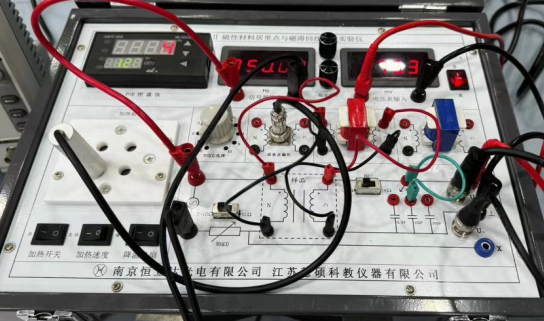
\includegraphics[clip,scale=0.9,trim={0 0 0 0}]{fig/fig10.png}
           	        \caption{Experimental Instrument Panel Wiring Diagram}
           	        \label{figure.1}
               \end{figure}    
	
	\begin{enumerate}
	    \item First, select sample 2 for the experiment. Refer to Figure and connect the circuit as shown in Figure. Place the selection switch of the sampling resistor \(R\) in the range of \(0~10\Omega\), the multi-range switch in the range of around \(6\Omega\), the selection switch in the range of \(R2\) select \(10k\Omega\), and the integral capacitor \(C\) select \(10uF\).
	    
	    \item Adjust the working mode of the oscilloscope display to X-Y mode, which is the graphical instrument mode.
	    
	    \item The input of the oscilloscope X is in AC mode, and the voltage of the sampling resistor \(R1\) is measured.
	    
	    \item The input of the oscilloscope Y is in DC mode, and the voltage of the integrated capacitor \(C\) is measured.
	    
	    \item Power on the oscilloscope and the experimental platform, set the signal source output frequency to \(50Hz\), and initially adjust the amplitude to \(0V\). At this point, the oscilloscope should display a centered bright spot. Gradually increase the magnetizing current by adjusting the amplitude knob of the signal source until the hysteresis loop is displayed on the oscilloscope, and the \(B\) value on the Y-axis slowly increases to saturation. Adjust the oscilloscope's Y sensitivity if necessary to obtain a clear and aesthetically pleasing hysteresis loop graph. If the graph is not centered, use the X and Y position knobs on the oscilloscope to make the image clear, symmetrical, and centered.
	    
	    \item Adjust the signal source amplitude knob to gradually reduce the magnetization current, and observe the hysteresis loop from large to small until it shrinks to a point, which is the demagnetization process.
	\end{enumerate}
	
	Mapping the basic magnetization curve and saturation hysteresis loop of ferromagnetic materials.
	\begin{enumerate}
	    \item Establish a coordinate system on Cartesian paper with \(X(H)\) as the horizontal axis and \(Y(B)\) as the vertical axis. Place the origin at the center of the paper, and ensure that the scale on the coordinate paper corresponds to the scale on the oscilloscope screen (you may adjust the scale for clarity).
	    
	    \item Starting from zero, gradually increase the magnetizing current to trace the hysteresis loop from small to large until saturation. Select 10 appropriate points along the loop, pause, and record their \(X, Y\) coordinates in Table 4.14-1. Mark the position of the positive end of the hysteresis loop on the coordinate paper, and smoothly connect these points to obtain the basic magnetization curve.
	    
	    \item In the same coordinate system, plot points first, and then connect them to depict the complete saturated hysteresis loop. Pay attention to accurately capturing the coordinates of key values. Record the sensitivity values (\(V/DIV\)) of the oscilloscope's \(X\) and \(Y\) axes; the sensitivity of the oscilloscope must remain constant throughout the experiment.
	\end{enumerate}
	
	Select sample 3 and repeat the above experimental steps. The signal frequency and values of $R_1$, $R_2$, and $C$ are the same as before, and their basic magnetization curve and saturation hysteresis loop are also obtained.
	
	Determine the Curie point by observing the temperature at which the hysteresis loop
	disappears.
	
	\begin{enumerate}
	    \item Circuit connection: Insert the probe end of the Curie point detection sample into the heating well, and the plug end into the aviation socket of sample 1 on the panel. Connect the circuit according to the circuit diagram shown in Figure, and select \(R1=51\Omega\), \(R2=1k\Omega\), \(C=0.33uF\), signal source frequency is \(30kHz\), amplitude is \(16V_{p-p}\). \(UH\) and \(UB\) are respectively connected to the "X input" and "Y input" of the oscilloscope, with the ground being the common terminal.
	    
	    \item Turn on the power switch of the experimental instrument and oscilloscope. At this point, the heating switch on the panel is turned off, adjust the oscilloscope appropriately, and display the hysteresis loop on the screen.
	    
	    \item Open the heating switch and set the heating speed to fast. Preheat the sample by presetting the temperature to \(80°C\) on the temperature controller. Once stabilized, incrementally increase the temperature in \(5°\) steps while observing the hysteresis loop on the oscilloscope. Record the temperature value displayed when the hysteresis loop disappears (becomes a single line); this is the measured Curie point temperature.
	\end{enumerate}
	
	After the measurement is completed, turn off the heating switch and turn on the cooling fan to cool the heating well. If time permits, it can be reheated when the temperature drops to $10 ^{\circ}C$ below the Curie point temperature just measured (at which point a hysteresis loop appears), and then measured again. The average of the two measurements is taken as the measurement result.
	
	Determine the Curie point by measuring the relationship curve of induced
	electromotive force with temperature change.
	
	\begin{enumerate}
	    \item The measurement line connection and parameter settings are the same as above, and the \(UB\) can be connected without an oscilloscope. Connect to the voltmeter input.
	    
	    \item At room temperature, set the temperature to \(15°C\) below the Curie point temperature measured above, turn on the heating switch to raise the temperature, wait for it to stabilize, and repeat \(5°C\) steps to heat the sample.
	    
	    \item Observe the changes in the voltmeter values during the heating process of the heating well, and record the induced electromotive force values at different temperatures in the table.
	\end{enumerate}
	
	The two contents can be carried out simultaneously, and the Curie point measurement of both methods can be completed in one heating process. Sample 1 is equipped with three probes with different Curie points, which can be selected according to the situation ($95^{\circ}C, 135^{\circ}C$ sample is recommended for experiments to save experimental time and avoid hot hands).
	
	\section{Data processing}
   \subsection{Mapping of the basic magnetization curve of ferrite}
   To obtain a visually appealing hysteresis loop on the oscilloscope screen, when measuring the basic magnetization curve of ferrite, first demagnetize the sample and then gradually increase the current from zero. Record the X and Y values of each hysteresis loop's vertex until saturation is reached.
   
       Oscilloscope X-axis sensitivity: $100mV$, Oscilloscope Y-axis sensitivity: $500mV$
       
   \begin{table}[htbp]
     \centering
     \caption{Relevant data}
       \begin{tabular}{lr}
       \toprule[2pt]
       notation & \multicolumn{1}{l}{numbers} \\
       \midrule
       $N_1$    & $50T$ \\
       $N_2$    & $150T $\\
       $R_1$    & $6\Omega $ \\
       $R_2$   & $10K\Omega$  \\
       $C $    & $10\mu F$ \\
       $L $    & $60mm$ \\
       $S  $   & $80mm^2$ \\
       \bottomrule[2pt]
       \end{tabular}%
     \label{tab:addlabel}%
   \end{table}%
   
  
   \begin{table}[htbp]
     \centering
     \caption{Mapping of the basic magnetization curve of ferrite}
       \begin{tabular}{lcccccccc}
       \toprule[2pt]
       Point & 1     & 2     & 3     & 4     & 5     & 6     & 7     & 8 \\
       \midrule
       $U_x$   & $20mV$    & $345mV$   & $445mV$   & $595mV$   & $757mV$   & $895mV$   & $1.07V$  & $1.23V$ \\
       $U_y$  & $500\mu V$   & $44.5mV$  & $92mV$    & $127mV$   & $167mV$   & $194mV$   & $217mV$   & $244mV$ \\
       \bottomrule[2pt]
       \end{tabular}%
     \label{tab:addlabel}%
   \end{table}%
   
  By calculating $U_H$ and $U_B$, substitute the values into the formula to calculate the values
  of $H$ and $B$, and then calculate $\mu = B/H$. Based on the calculated data, the basic
  magnetization curve $( B - H )$ and $\mu - H$ curve of the sample can be plotted.
    
         \begin{figure}[H]
               	    	\centering
               	    	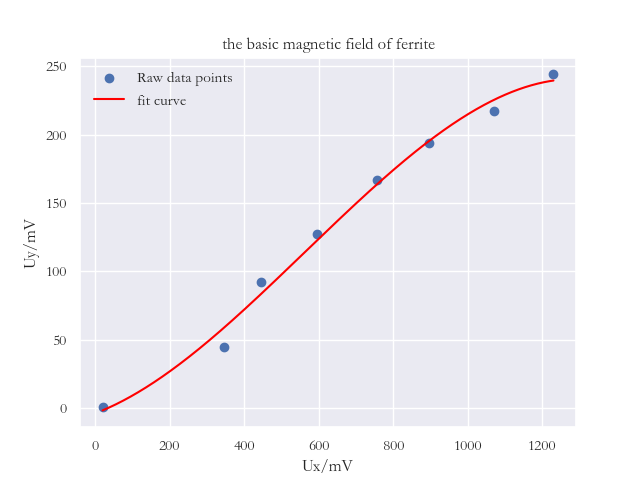
\includegraphics[clip,scale=0.9,trim={0 0 0 0}]{fig/fig11.png}
               	        \caption{the basic magnetic field of ferrite}
               	        \label{figure.1}
                   \end{figure}   
   
   \subsection{Plotting the dynamic hysteresis loop}
   Display a visually appealing hysteresis loop on the oscilloscope and measure the number of grids corresponding to different points on the hysteresis loop. Then, fill in the data in Table. The coordinate readings in each direction correspond to two Y- coordinate readings (one after saturation). Refer to the data recorded in the table, and ensure that there are more data points in areas where the curve's slope is stee
   \begin{table}[htbp]
     \centering
     \caption{Plotting the dynamic hysteresis loop}
       \begin{tabular}{lcccccc}
       \toprule[2pt]
       Point & \multicolumn{1}{l}{1($H_s , B_s$)} & 2     & \multicolumn{1}{l}{3($0, B_r$)} & 4     & \multicolumn{1}{l}{5($−H_c , 0$)} & 6 \\
       \midrule
       $U_x$   & 1.23V  & 482mV   & 20mV    & -292mV  & -455mV  & -617mV \\
       $U_y$   & 244mV   & 190mV   & 144mV   & 66.5mV  & -0.5mV  & -111mV \\
       \bottomrule[1.5pt]
       Point & \multicolumn{1}{l}{7($-H_s , −B_s$)} & 8     & \multicolumn{1}{l}{9($0, −B_r$)} & 10    & \multicolumn{1}{l}{11($H_c , 0$)} & 12 \\
       \midrule
       $U_x$   & -1.24V & -355mV & 20mV    & 382mV   & 495mV   & 757mV \\
       $U_y$   & -250mV  & -198mV  & -153mV  & -78.5mV & -0.5mV  & 126mV \\
       \bottomrule[2pt]
       \end{tabular}%
     \label{tab:addlabel}%
   \end{table}%
   
   Derive the dynamic hysteresis loop:
            \begin{figure}[H]
                  	    	\centering
                  	    	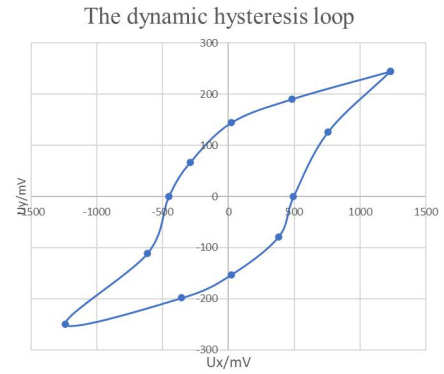
\includegraphics[clip,scale=1.2,trim={0 0 0 0}]{fig/fig12.png}
                  	        \caption{the dynamic hysteresis loop}
                  	        \label{figure.1}
                      \end{figure}  
                      
   Record that the Coercive force $H_c = 475mV$, remanence $B_r = 148mV$, saturation magnetic induction $B_m = 247mV$
   
   \subsection{Measuring the Curie point of the sample}
  Change the sample to sample 1, adjust the parameters and heat up, record the temperature corresponding to the disappearance of hysteresis loop.
  \begin{table}[htbp]
    \centering
    \caption{Add caption}
      \begin{tabular}{lcccc}
      \toprule[2pt]
      Times & 1     & 2     & 3     & \multicolumn{1}{l}{Average Value} \\
      \midrule
      $T_c / ^{\circ}C $    & 101   & 103   & 100   & 101.33 \\
      \bottomrule[2pt]
      \end{tabular}%
    \label{tab:addlabel}%
  \end{table}%
  
  Calculate the average temperature corresponding to the disappearance of hysteresis loop:
  \begin{eqnarray}
  \overline{\mathrm{T}}=\frac{1}{\mathrm{n}} \sum_{\mathrm{i}=1}^{\mathrm{n}} \mathrm{T}_{\mathrm{i}}=101.33
  \end{eqnarray}
  Calculate the standard deviation for the temperature:
  \begin{eqnarray}
  \sigma=\sqrt{\frac{\sum_{\mathrm{i}=1}^{\mathrm{n}}\left(\mathrm{T}_{\mathrm{i}}-\mathrm{T}\right)}{\mathrm{n}-1}}=1.52
  \end{eqnarray}
  Distinguish abnormal data according to the Grabbs criterion. Take significance level $a=0.01$, measurement frequency$ n=5$, and check the critical value in the comparison table $g_0(5, 0.01)=1.155$, Take $\Delta T_i$ to calculate $g_i$ value.
  \begin{eqnarray}
  \mathrm{g}_{1}=\frac{\Delta \mathrm{T}_{1}}{\sigma}=0.22\\
  \mathrm{g}_{2}=\frac{\Delta \mathrm{T}_{2}}{\sigma}=1.09\\
  \mathrm{g}_{3}=\frac{\Delta \mathrm{T}_{3}}{\sigma}=0.88\\
  \end{eqnarray}
  Determine that there is no abnormal data.
  
  The measurement result is represented as:
  \begin{eqnarray}
  \mathrm{T}=101.33 \pm 1.52 
  \end{eqnarray}

\section{Conclusion and analysis}
\subsection{Conclusion}
\begin{itemize}
    \item Through the observation of hysteresis loops on the oscilloscope, the Curie point temperature of the tested ferromagnetic material was determined by \(T = 101.33 \pm 1.52\).
    \item The hysteresis loop provided insights into the magnetic characteristics, including the Coercive force \(H_c = 475 \, \text{mV}\), remanence \(B_r = 148 \, \text{mV}\), and saturation magnetic induction \(B_m = 247 \, \text{mV}\).
    \item The process involved heating the sample gradually, monitoring the changes in the hysteresis loop, and identifying the temperature at which the loop disappeared, indicating the Curie point.
    \item The experiment demonstrated the dynamic magnetic properties and hysteresis behavior of ferromagnetic materials, essential for understanding their magnetic behavior and applications.
\end{itemize}


\subsection{Error analysis}
\begin{itemize}
    \item \textbf{Curie Point Temperature Measurement:}
    \begin{itemize}
        \item \textbf{Observation Error:} The precision of the oscilloscope in reading hysteresis loops may introduce slight variations. The Curie point temperature \(T = 101.33 \pm 1.52\) is subject to potential observational inaccuracies.
    \end{itemize}
    
    \item \textbf{Magnetic Characteristics:}
    \begin{itemize}
        \item \textbf{Instrumental Error:} The values for coercive force (\(H_c\)), remanence (\(B_r\)), and saturation magnetic induction (\(B_m\)) (\(H_c = 475 \, \text{mV}\), \(B_r = 148 \, \text{mV}\), \(B_m = 247 \, \text{mV}\)) are influenced by equipment precision and calibration.
    \end{itemize}
    
    \item \textbf{Experimental Procedure:}
    \begin{itemize}
        \item \textbf{Heating Process Variability:} The gradual heating process introduces uncertainties in pinpointing the exact temperature at which the hysteresis loop disappears. Variations in the heating rate and environmental conditions may contribute to this uncertainty.
    \end{itemize}
    
    \item \textbf{General Considerations:}
    \begin{itemize}
        \item \textbf{Material Homogeneity:} Inherent variations in the ferromagnetic material's composition and homogeneity can impact the accuracy of the experiment.
    \end{itemize}
\end{itemize}


\begin{appendix}
 \section{Experimental data recording graph} 
     	\begin{figure}[H]
     	    	\centering
     	    	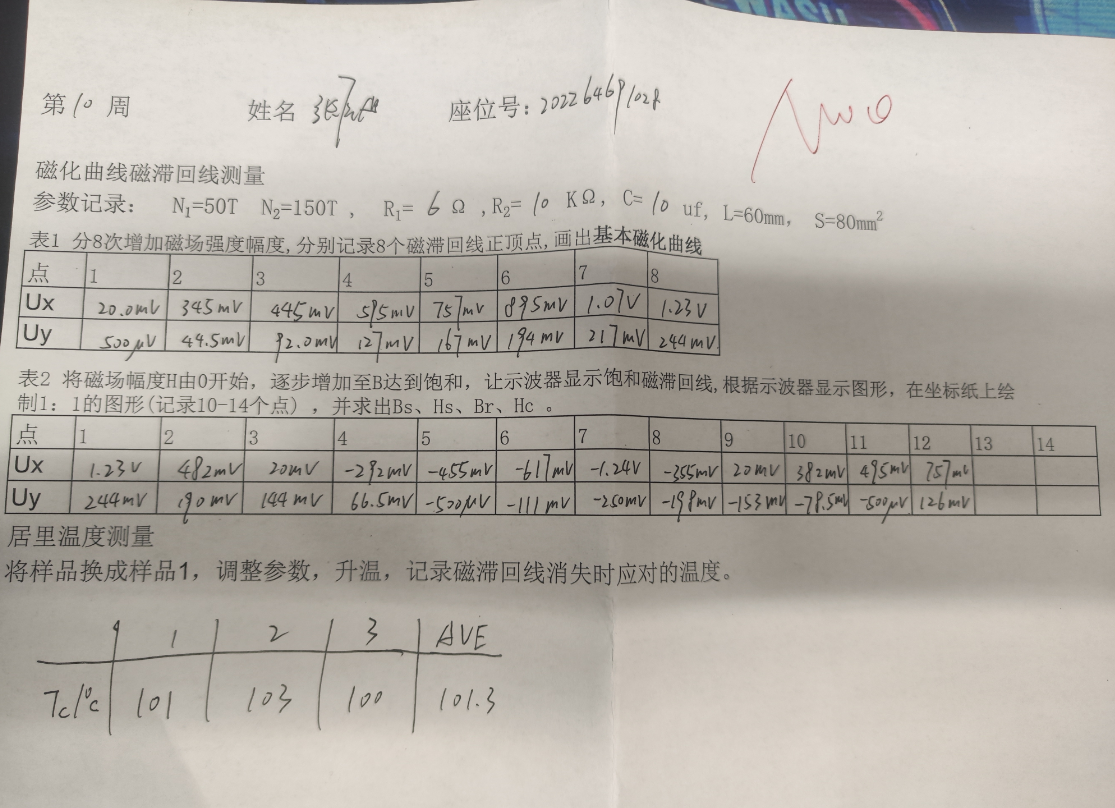
\includegraphics[clip,scale=0.8,trim={0 0 0 0}]{fig/fig13.png}
     	        \caption{Experimental data recording graph}
     	        \label{figure.19}
         \end{figure} 
 \end{appendix}        
\end{document}  